\appendix
\section{Appendix}

\subsection{Data}

\subsubsection{Data access}

Data was obtained from the Sentinel Stroke National Audit (SSNAP\footnote{https://www.strokeaudit.org/}), managed through the Healthcare Quality Improvement Partnership (HQIP\footnote{https://www.hqip.org.uk/}). SSNAP has near-complete coverage of all acute stroke admissions in the UK (outside Scotland). All hospitals admitting acute stroke participate in the audit, and year-on-year comparison with Hospital Episode Statistics\footnote{https://digital.nhs.uk/data-and-information/data-tools-and-services/data-services/hospital-episode-statistics} confirms estimated case ascertainment of 95\% of coded cases of acute stroke.

The NHS Health Research Authority decision tool\footnote{http://www.hra-decisiontools.org.uk/research/} was used to confirm that ethical approval was not required to access the data. Data access was authorised by HQIP (reference HQIP303). 

Data was retrieved for 246,676 emergency stroke admissions to acute stroke teams in England and Wales between 2016 and 2018 (three full years). 88,928 patients arrived within 4 hours of known stroke onset.

\subsubsection{Data fields}

\paragraph{Stroke Team}

\begin{itemize}
\item \emph{StrokeTeam}: Pseudonymised SSNAP `routinely admitting team` unique
  identifier. For emergency care it is expected that each hospital has
  one stroke team (though post-72 hour care may be reported under a
  different team at that hospital).
\end{itemize}

\paragraph{Patient -- general}

\begin{itemize}
\item  \emph{Pathway}: Total number of team transfers, excluding community teams
\item \emph{S1AgeOnArrival}: Age on arrival aggregated to 5 year bands
\item \emph{MoreEqual80y}: Whether the patient is \textgreater= 80 years old at the
  moment of the stroke
\item \emph{S1Gender}: Gender
\item \emph{S1Ethnicity}: Patient Ethnicity. Aggregated to White, Black, Mixed,
  Asian and Other
\end{itemize}


\paragraph{Patient -- pathway information}

\begin{itemize}
\item \emph{S1OnsetInHospital}: Whether the patient was already an inpatient at the
  time of stroke
\item \emph{S1OnsetToArrival\_min}: Time from symptom onset to arrival at hospital
  in minutes, where known and if out of hospital stroke
\item \emph{S1OnsetDateType}: Whether the date of onset given is precise, best
  estimate or if the stroke occurred while sleep
\item \emph{S1OnsetTimeType}: Whether the time of symptom onset given is precise,
  best estimate, not known
\item \emph{S1ArriveByAmbulance}: Whether the patient arrived by ambulance
\item \emph{S1AdmissionHour}: Hour of arrival, aggregates to 3 hour epochs
\item \emph{S1AdmissionDay}: Day of week at the moment of admission
\item \emph{S1AdmissionQuarter}: Year quarter (Q1: Jan-Mar; Q2:April-Jun; Q3:
  Jul-Sept; Q4: Oct-Dec)
\item \emph{S1AdmissionYear}: Year of admission
\item \emph{S2BrainImagingTime\_min}: Time from Clock Start to brain scan. In
  minutes. ``Clock Start'' is used throughout SSNAP reporting to refer
  to the date and time of arrival at first hospital for newly arrived
  patients, or to the date and time of symptom onset if patient already
  in hospital at the time of their stroke.
\item \emph{S2ThrombolysisTime\_min}: Time from Clock Start to thrombolysis. In
  minutes. ``Clock Start'' is used throughout SSNAP reporting to refer
  to the date and time of arrival at first hospital for newly arrived
  patients, or to the date and time of symptom onset if patient already
  in hospital at the time of their stroke.
\end{itemize}

\paragraph{Patient -- comorbidities}

\begin{itemize}
\item \emph{CongestiveHeartFailure}: Pre-Stroke Congestive Heart Failure
\item \emph{Hypertension}: Pre-Stroke Systemic Hypertension
\item \emph{AtrialFibrillation}: Pre-Stroke Atrial Fibrillation (persistent,
  permanent, or paroxysmal)
\item \emph{Diabetes}: Comorbidities: Pre-Stroke Diabetes Mellitus
\item \emph{StrokeTIA}: Pre-Stroke history of stroke or Transient Ischaemic Attack
  (TIA)
\item \emph{AFAntiplatelet}: Only available if ``Yes'' to Atrial Fibrillation
  comorbidity. Whether the patient was on antiplatelet medication prior
  to admission
\item \emph{AFAnticoagulent}: Prior to 01-Dec-2017: Only available if ``Yes'' to
  Atrial Fibrillation comorbidity; From 01-Dec-2017: available even if
  patient is not in Atrial Fibrillation prior to admission. Whether the
  patient was on anticoagulant medication prior to admission
\item \emph{AFAnticoagulentVitK}: If the patient was receiving anticoagulant
  medication, was it vitamin K antagonists
\item \emph{AFAnticoagulentDOAC}: If the patient was receiving anticoagulant
  medication, was it direct oral anticoagulants (DOACs)
\item \emph{AFAnticoagulentHeparin}: If the patient was receiving anticoagulant
  medication, was it Heparin
\end{itemize}

\paragraph{Patient -- NIH Stroke Scale}

\begin{itemize}
\item \emph{S2NihssArrival}: National Institutes of Health Stroke Scale score on
  arrival at hospital
\item \emph{BestGaze}: National Institutes of Health Stroke Scale Item 2 Best Gaze
  (higher values indicate more severe deficit)
\item \emph{BestLanguage}: National Institutes of Health Stroke Scale Item 9 Best
  Language (higher values indicate more severe deficit)
\item \emph{Dysarthria}: National Institutes of Health Stroke Scale Item 10
  Dysarthria (higher values indicate more severe deficit)
\item \emph{ExtinctionInattention}: National Institutes of Health Stroke Scale Item
  11 Extinction and Inattention (higher values indicate more severe
  deficit)
\item \emph{FacialPalsy}: National Institutes of Health Stroke Scale Item 4 Facial
  Paresis (higher values indicate more severe deficit)
\item \emph{LimbAtaxia}: National Institutes of Health Stroke Scale Item 7 Limb
  Ataxia (higher values indicate more severe deficit)
\item \emph{Loc}: National Institutes of Health Stroke Scale Item 1a Level of
  Consciousness (higher values indicate more severe deficit)
\item \emph{LocCommands}: National Institutes of Health Stroke Scale Item 1c Level
  of Consciousness Commands (higher values indicate more severe deficit)
\item \emph{LocQuestions}: National Institutes of Health Stroke Scale Item 1b Level
  of Consciousness Questions (higher values indicate more severe
  deficit)
\item \emph{MotorArmLeft}: National Institutes of Health Stroke Scale Item 5a Motor
  Arm - Left (higher values indicate more severe deficit)
\item \emph{MotorArmRight}: National Institutes of Health Stroke Scale Item 5b
  Motor Arm - Right (higher values indicate more severe deficit)
\item \emph{MotorLegLeft}: National Institutes of Health Stroke Scale Item 6a Motor
  Leg - Left (higher values indicate more severe deficit)
\item \emph{MotorLegRight}: National Institutes of Health Stroke Scale Item 6b
  Motor Leg - Right (higher values indicate more severe deficit)
\item \emph{Sensory}: National Institutes of Health Stroke Scale Item 8 Sensory
  (higher values indicate more severe deficit)
\item \emph{Visual}: National Institutes of Health Stroke Scale Item 3 Visual
  Fields (higher values indicate more severe deficit)
\end{itemize}

\paragraph{Patient -- other clinical features}

\begin{itemize}
\item \emph{S2INR}: Patient's International Normalised ratio (INR) on arrival at
  hospital (available since 01-Dec-2017)
\item \emph{S2INRHigh}: INR was greater than 10 on arrival at hospital (available
  since 01-Dec-2017)
\item \emph{S2INRNK}: INR not checked (available since 01-Dec-2017)
\item \emph{S2NewAFDiagnosis}: Whether a new diagnosis of Atrial Fibrillation was
  made on admission
\item \emph{S2RankinBeforeStroke}: Patient's modified Rankin Scale score before
  this stroke (Higher values indicate more disability)
\item \emph{S2StrokeType}: Whether the stroke type was infarction or primary
  intracerebral haemorrhage
\item \emph{S2TIAInLastMonth}: Whether the patient had a Transient Ischaemic Attack
  during the last month. Item from the SSNAP comprehensive dataset
  questions (not mandatory)
\end{itemize}

\paragraph{Patient -- thrombolysis given}

\begin{itemize}
\item \emph{S2Thrombolysis}: Whether the patient was given thrombolysis (clot
  busting medication)
\end{itemize}

\paragraph{Patient -- reason stated for not giving thrombolysis}

\begin{itemize}
\item \emph{Age}: If the answer to thrombolysis given was ``no but'', the reason
  was Age
\item \emph{Comorbidity}: If the answer to thrombolysis given was ``no but'', the
  reason was Co-morbidity
\item \emph{Haemorrhagic}: If the answer to thrombolysis given was ``no but'', the
  reason was Haemorrhagic stroke
\item \emph{Improving}: If the answer to thrombolysis given was ``no but'', the
  reason was Symptoms Improving
\item \emph{Medication}: If the answer to thrombolysis given was ``no but'', the
  reason was Medication
\item \emph{OtherMedical}: If the answer to thrombolysis given was ``no but'', the
  reason was Other medical reason
\item \emph{Refusal}: If the answer to thrombolysis given was ``no but'', the
  reason was Refusal
\item \emph{TimeUnknownWakeUp}: If the answer to thrombolysis given was ``no but'',
  the reason was Symptom onset time unknown/wake-up stroke
\item \emph{TimeWindow}: If the answer to thrombolysis given was ``no but'', the
  reason was Age
\item \emph{TooMildSevere}: If the answer to thrombolysis given was ``no but'', the
  reason was Stroke too mild or too severe
\end{itemize}



%%%%%%%%%%%%%%%%%%%%%%%%%%%%%%%%%%%%%%%%%%%%%%%%%%%%%%%%%%%%%%%%%%%%%%%%%%%

\subsection{Probability, odds, and Shap values (log odds shifts): A brief explanation}

Many of us find it easiest to think of the chance of something occurring
as a probability. For example, there might be a probability of 10\% that
it will rain today. That is the same as saying there will be one rainy
day out of ten days for days with this given probability of rain.

In our stroke thrombolysis model, Shap values tell us how knowing
something particular about a patient (such as the patient
\emph{feature}, `Is their stroke caused by a clot or a bleed?') adjusts
our prediction of whether they will receive thrombolysis or not.

This is made a little more complicated for us because Shap is usually
reported as a \emph{log odds shift}. It is useful for us to see how
those relate to probabilities, and get a sense of how significant Shap
values in the range of 0.5 to 5 (or -0.5 to -5) are, as that is a common
range of Shap values that we will see in our models.

\subsubsection{Probability}

We will take the example that Shap reports that a model's base
probability prediction, before the contribution of features is 0.25, or
a 25\% probability of receiving thrombolysis; that is 1 in 4 patients
with this prediction would be expected to receive thrombolysis.

\subsubsection{Odds}

\emph{Probability} expresses the chance of something happening as the
number of positive occurrences as a fraction of all occurrences
(i.e.~the number of patients receiving thrombolysis as a fraction of the
total number of patients).

\emph{Odds} express the chance of something happening as the ratio of
the number of positive occurrences (i.e.~receiving thrombolysis) to the
number of negative occurrences (i.e.~\emph{not} receiving thrombolysis).

If we have probability prediction of 0.25 would receive thrombolysis,
that would mean 1 in 4 of those patients receive thrombolysis. Expressed
as odds, for every one patient that receives thrombolysis, three will
not. The odds are expressed as 1:3 or 1/3. This may also be calculated
as a decimal (1 divided by 3), 0.333.

Odds (O) and probability (P) may be converted with the following
equations:

\begin{enumerate}
\def\labelenumi{(\arabic{enumi})}
\item
  O = P / (1 - P)
\item
  P = O / (1 + O)
\end{enumerate}

\subsubsection{Shap values: Log odds shifts}

Here we will calculate the effect of Shap values, and try and build some
intuition on the size of effect Shap values of 0.5 to 5 give (we will
look at positive and negative Shap values).

Shap usually outputs the effect of a particular feature in how much it
shifts the odds. For reasons we will not go into here, that shift (which
is the `Shap value') is usually given in `log odds' (the logarithm of
the odds value). For the mathematically inclined, we use the natural log
(\emph{ln}).

Let's look at some Shap values (log odds) and see how much they change
the odds of receiving thrombolysis.

First we'll look at the shift in odds the Shap values give. This is
calculated as \emph{shift = exp(Shap)} (table \ref{tab:odds_1}).

\begin{longtable}[]{@{}ll@{}}
\caption{The relationship between \emph{odds} and \emph{log odds}.}\\
\toprule
SHAP (log odds) & Shift in odds (multiply original odds)\tabularnewline
\midrule
\endhead
0.5 & 1.65\tabularnewline
1 & 2.72\tabularnewline
2 & 7.39\tabularnewline
3 & 20.1\tabularnewline
4 & 54.6\tabularnewline
5 & 148\tabularnewline
\bottomrule
\label{tab:odds_1}
\end{longtable}

\emph{Positive Shap values: worked example}

Now let us work through an example of starting with a known baseline
\emph{probability} (before we consider what we know about a particular
patient feature), converting that to \emph{odds}, applying a Shap
\emph{log odds shift} for that particular feature, and converting back
to \emph{probability} after we have applied the influence of that
feature.

The the effects of those shifts on our baseline probability of 0.25 are shown in table \ref{tab:odds_2}.

\begin{longtable}[]{@{}llllll@{}}
\caption{The effect of SHAP values between 0.5 and 5 on a base probability of 0.25}\\
\toprule
Starting P & Starting O & SHAP & Shift (multiply O) & Shifted O &
Shifted P (\%)\tabularnewline
\midrule
\endhead
0.25 (25\%) & 0.333 & 0.5 & 1.65 & 0.550 & 0.3547
(35.5\%)\tabularnewline
0.25 (25\%) & 0.333 & 1 & 2.72 & 0.907 & 0.4754 (47.5\%)\tabularnewline
0.25 (25\%) & 0.333 & 2 & 7.39 & 2.46 & 0.7112 (71.1\%)\tabularnewline
0.25 (25\%) & 0.333 & 3 & 20.1 & 6.70 & 0.8700 (87.0\%)\tabularnewline
0.25 (25\%) & 0.333 & 4 & 54.6 & 18.2 & 0.9479 (94.8\%)\tabularnewline
0.25 (25\%) & 0.333 & 5 & 148 & 49.5 & 0.9802 (98.0\%)\tabularnewline
\bottomrule
\label{tab:odds_2}
\end{longtable}

So, for example, a Shap value of 0.5 for one particular feature tells us
that that particular feature in that patient shifts our expected
probability of that patient receiving thrombolysis from 25\% to 36\%. A
Shap value of 5 for the same feature would shift the probability of that
patient receiving thrombolysis up to 98\%.

\emph{Negative Shap values: worked example}

If we have a negative Shap value then odds are reduced (a Shap of -1
will lead to the odds being divided by 2.72, which is the same as
multiplying by 1/2.72, which is 0.3679), as shown in table \ref{tab:odds_3}.

\begin{longtable}[]{@{}llllll@{}}
\caption{The effect of SHAP values between -0.5 and -5 on a base probability of 0.25}\\
\toprule
Starting P & Starting O & Shap & Shift (multiply O) & Shifted O &
Shifted P\tabularnewline
\midrule
\endhead
0.25 (25\%) & 0.333 & -0.5 & 0.6065 & 0.2022 & 0.1682
(16.8\%)\tabularnewline
0.25 (25\%) & 0.333 & -1 & 0.3679 & 0.1226 & 0.1092
(10.9\%)\tabularnewline
0.25 (25\%) & 0.333 & -2 & 0.1353 & 0.0451 & 0.0432
(4.32\%)\tabularnewline
0.25 (25\%) & 0.333 & -3 & 0.0498 & 0.0166 & 0.0163
(1.63\%)\tabularnewline
0.25 (25\%) & 0.333 & -4 & 0.0183 & 0.0061 & 0.0061
(0.61\%)\tabularnewline
0.25 (25\%) & 0.333 & -5 & 0.0067 & 0.0022 & 0.0022
(0.22\%)\tabularnewline
\bottomrule
\label{tab:odds_3}
\end{longtable}

So, for example, a Shap value of -0.5 for one particular feature tells
us that that particular feature in that patient shifts our expected
probability of that patient receiving thrombolysis from 25\% to 17\%. A
Shap value of 5 for the same feature would shift the probability of that
patient receiving thrombolysis down to 2\%.

\subsubsection{Observations about Shap values}

We begin to get some intuition on Shap values. A Shap value of 0.5 (or
-0.5) leads to a small, but still noticeable, change in probability.
Shap values of 5 or -5 have effectively pushed probabilities to one
extreme or the other.

%%%%%%%%%%%%%%%%%%%%%%%%%%%%%%%%%%%%%%%%%%%%%%%%%%%%%%%%%%%%%%%%%%%%%%%%%%%%%%%%%%%%%%%
\subsection{Machine learning methods}

All work was conducted in Python (v3.8). All code is available at: \url{https://github.com/samuel-book/samuel_shap_paper_1}.

Our machine learning model used XGBoost (\emph{eXtreme Gradient Boosting}, v1.5, \url{https://pypi.org/project/xgboost/}). We used default settings apart from *learning rate* was set at 0.5 (see section below on \emph{'Fine-tuning of model regularisation'}.

Machine learning models were explained using SHAP (\emph{SHapley Additive exPlanations}, v0.41 \url{https://pypi.org/project/shap/}). 
%%%%%%%%%%%%%%%%%%%%%%%%%%%%%%%%%%%%%%%%%%%%%%%%%%%%%%%%%%%%%%%%%%%%%%%%%%%%%%%%%%%%%%%

\subsection{Feature selection}

A simplified model was created by using \emph{forward feature selection} where features were added in accordance to how much each one improved the Receiver Operating Characteristic (ROC) Area Under Curve (AUC). ROC AUC was measured using stratified k-fold validation (k=5). A model with all available 84 features had an ROC AUC of 0.922. A model with 10 features had an ROC AUC of 0.0.919.

The 10 features selected (figure \ref{fig:feature_selection}) were:

\begin{itemize}
    \item \emph{Arrival-to-scan time}: Time from arrival at hospital to scan (mins)
    \item \emph{Infarction}: Stroke type (1 = infarction, 0 = haemorrhage)
    \item \emph{Stroke severity}: Stroke severity (NIHSS) on arrival
    \item \emph{Precise onset time}: Onset time type (1 = precise, 0 = best estimate)
    \item \emph{Prior disability level}: Disability level (modified Rankin Scale) before stroke
    \item \emph{Stroke team}: Stroke team attended
    \item \emph{Use of AF anticoagulants}: Use of atrial fibrillation anticoagulant (1 = Yes, 0 = No)
    \item \emph{Onset-to-arrival time}: Time from onset of stroke to arrival at hospital (mins)
    \item \emph{Onset during sleep}: Did stroke occur in sleep?
    \item \emph{Age}: Age (as middle of 5 year age bands)
\end{itemize}

\begin{figure}
\centering
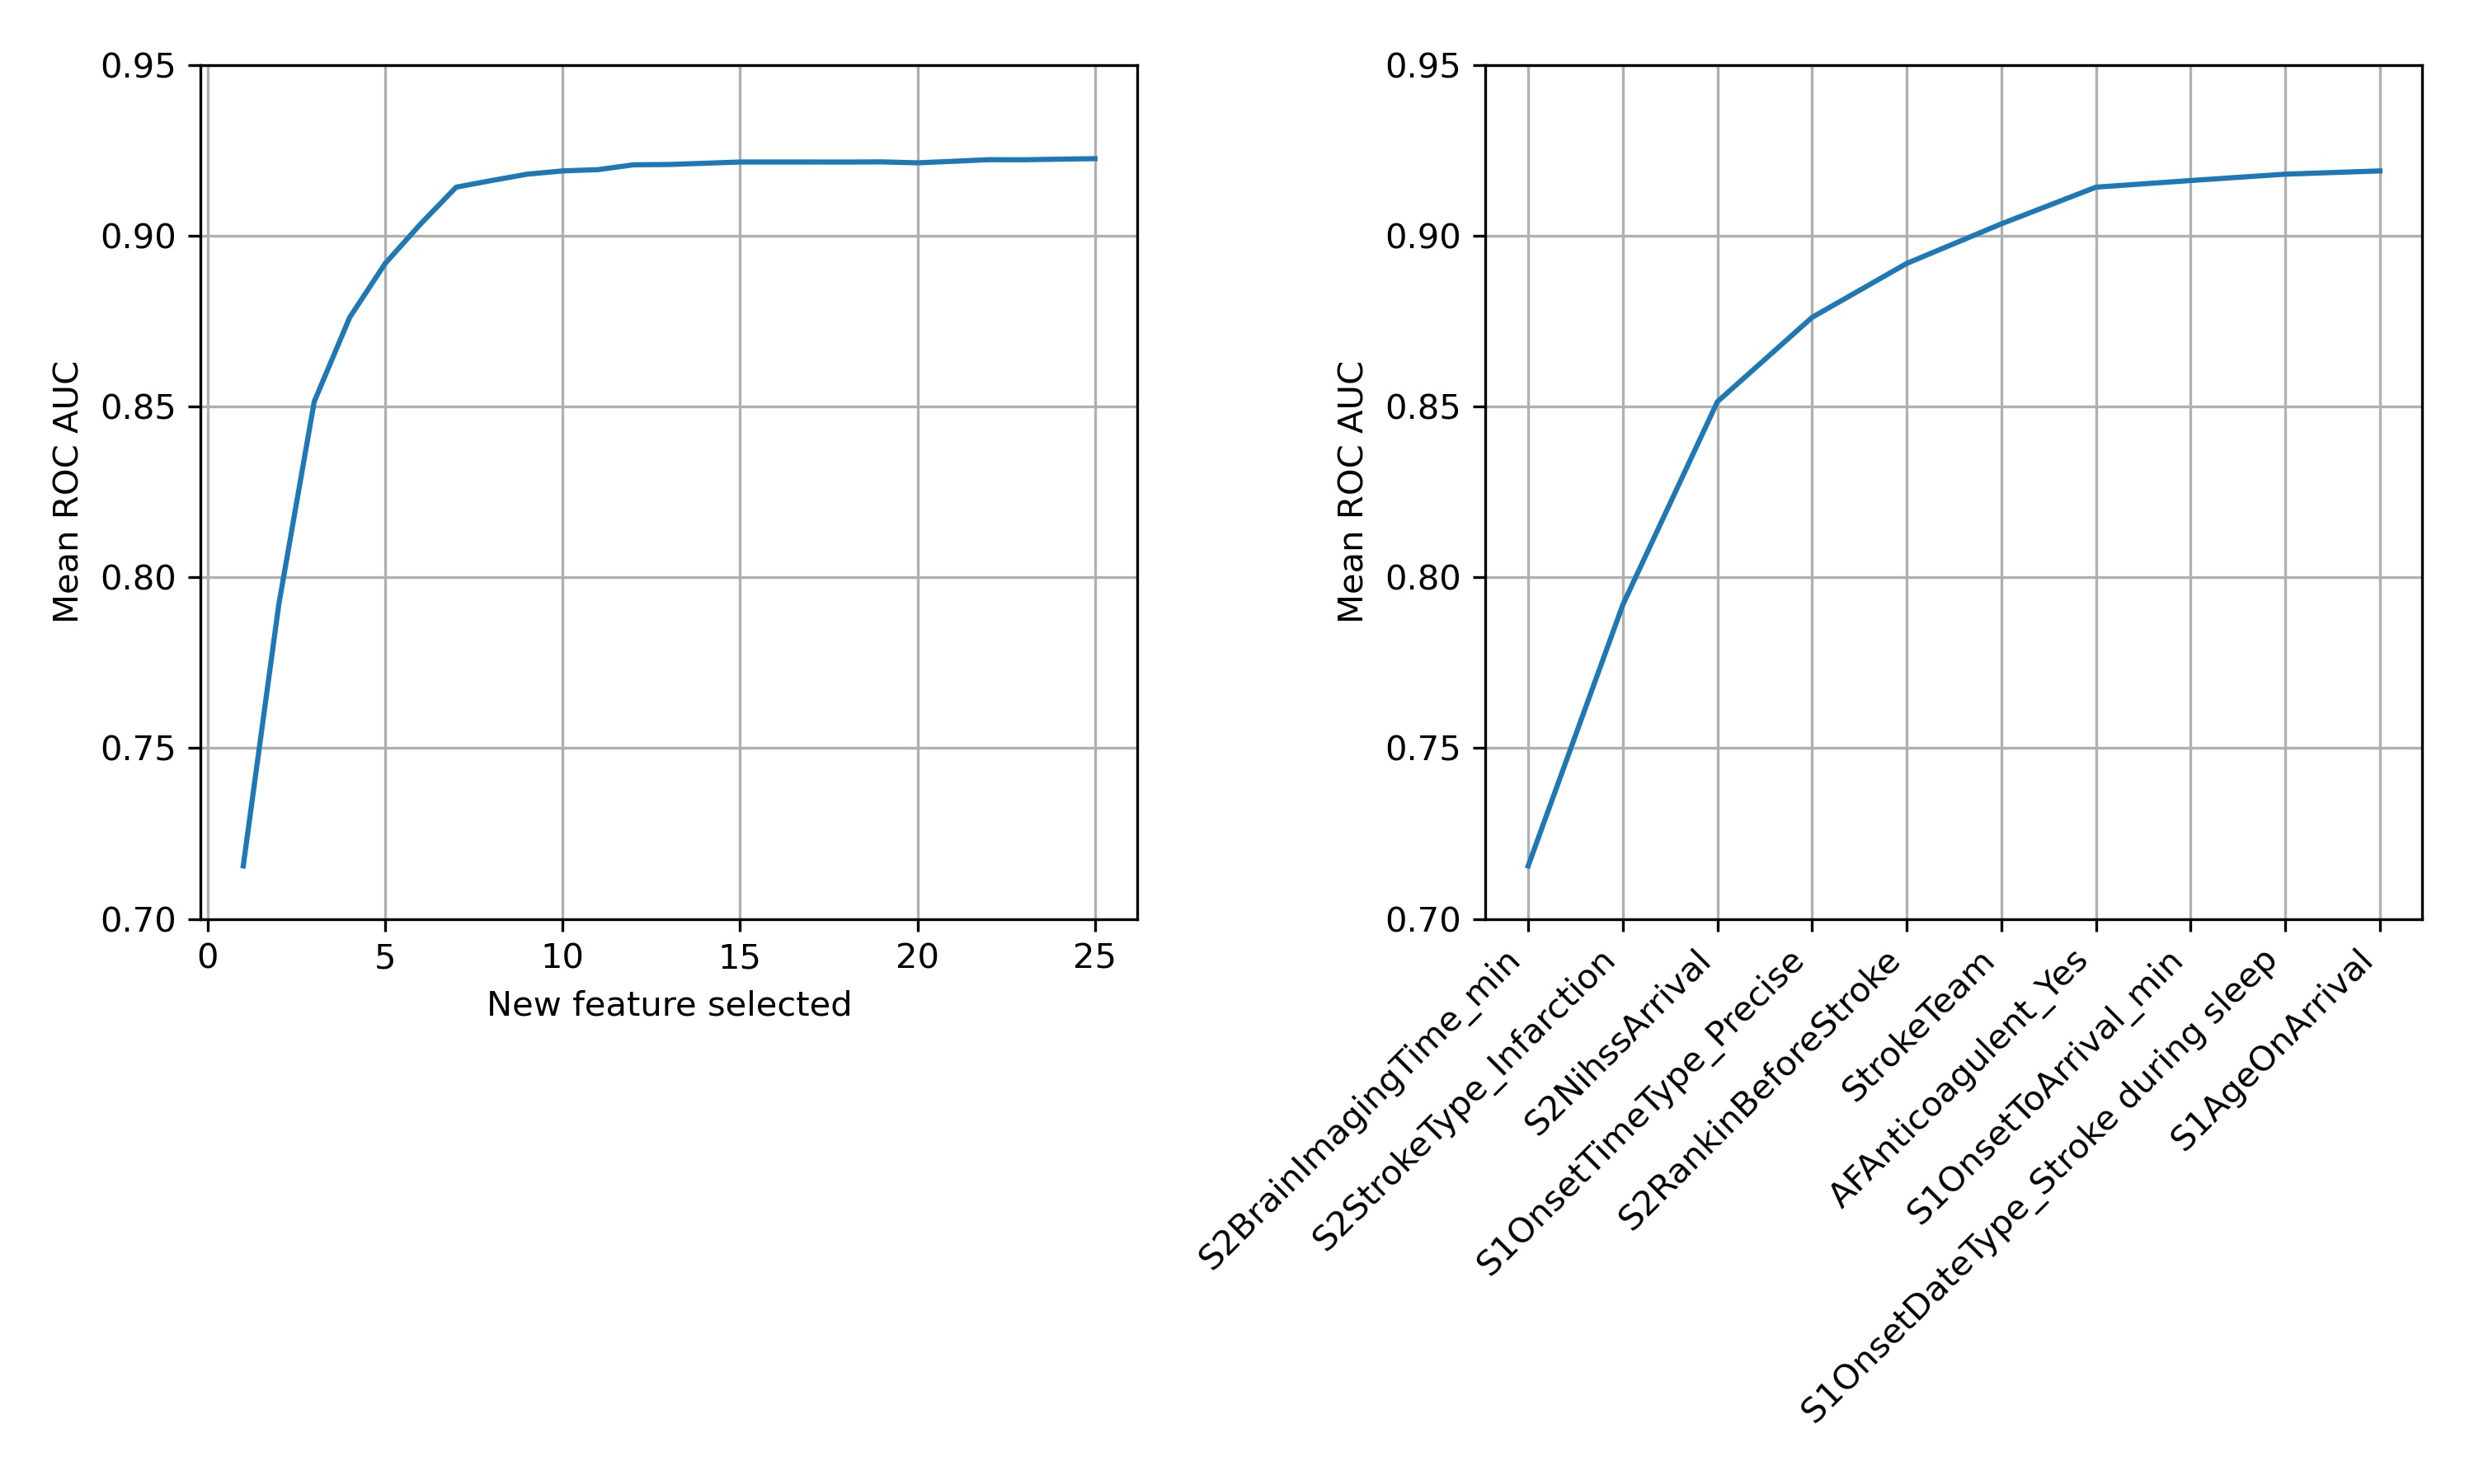
\includegraphics[width=1\textwidth]{./images/01_feature_selection}
\caption{The effect of increasing the number of features on model accuracy measured by Receiver Operating Characteristic (ROC) Area Under Curve (AUC). Left: Improvement with ROC AUC with selection of up to 25 features. Right: Improvement with ROC AUC with selection of the best 10 features. ROC was measured with stratified 5-fold cross-validation. Results show the mean of the 5-fold replicates.}
\label{fig:feature_selection}
\end{figure}

All results from this point forward will use the 10 feature model.

%%%%%%%%%%%%%%%%%%%%%%%%%%%%%%%%%%%%%%%%%%%%%%%%%%%%%%%%%%%%%%%%%%%%%%%%%%%%%%%%%%%%%%%

\subsection{Correlations within the 10 selected features}

Correlations between the 10 features were measured using coefficients of determination (r-squared). All r-squared were less than 0.15, and all r-squared were less than 0.05 except 1) age and prior disability level (r-squared 0.146), and 2) onset during sleep and precise onset time (r-squared 0.078). All correlations are shown in table \ref{tab:correl}.

\begin{longtable}[]{@{}rrr@{}}
\caption{Correlations between the 10 features selected for the XGBoost machine learning model.}\\
\toprule
variable 1 & Variable 2 & r-squared\tabularnewline
\midrule
\endhead
Age & Prior disability level & 0.1462\tabularnewline
Onset during sleep & Precise onset time & 0.0784\tabularnewline
Stroke severity & Prior disability level & 0.0454\tabularnewline
Stroke severity & Infarction & 0.0386\tabularnewline
Precise onset time & Onset-to-arrival time & 0.0344\tabularnewline
Stroke severity & Age & 0.0268\tabularnewline
Age & Use of AF anticoagulants & 0.0207\tabularnewline
Stroke severity & Onset-to-arrival time & 0.0186\tabularnewline
Precise onset time & Prior disability level & 0.0131\tabularnewline
Age & Precise onset time & 0.0090\tabularnewline
Prior disability level & Use of AF anticoagulants &
0.0070\tabularnewline
Onset during sleep & Onset-to-arrival time & 0.0043\tabularnewline
Onset-to-arrival time & Age & 0.0038\tabularnewline
Use of AF anticoagulants & Infarction & 0.0033\tabularnewline
Prior disability level & Onset-to-arrival time & 0.0022\tabularnewline
Precise onset time & Arrival-to-scan time & 0.0021\tabularnewline
Use of AF anticoagulants & Stroke severity & 0.0019\tabularnewline
Arrival-to-scan time & Stroke severity & 0.0019\tabularnewline
Precise onset time & Use of AF anticoagulants & 0.0016\tabularnewline
Stroke severity & Onset during sleep & 0.0011\tabularnewline
Infarction & Onset-to-arrival time & 0.0007\tabularnewline
Infarction & Onset during sleep & 0.0007\tabularnewline
Infarction & Precise onset time & 0.0006\tabularnewline
Onset-to-arrival time & Arrival-to-scan time & 0.0004\tabularnewline
Arrival-to-scan time & Prior disability level & 0.0001\tabularnewline
Onset-to-arrival time & Use of AF anticoagulants & 0.0001\tabularnewline
Stroke severity & Precise onset time & 0.0000\tabularnewline
Arrival-to-scan time & Age & 0.0000\tabularnewline
Use of AF anticoagulants & Onset during sleep & 0.0000\tabularnewline
Prior disability level & Onset during sleep & 0.0000\tabularnewline
Infarction & Age & 0.0000\tabularnewline
Use of AF anticoagulants & Arrival-to-scan time & 0.0000\tabularnewline
Onset during sleep & Arrival-to-scan time & 0.0000\tabularnewline
Arrival-to-scan time & Infarction & 0.0000\tabularnewline
Age & Onset during sleep & 0.0000\tabularnewline
Prior disability level & Infarction & 0.0000\tabularnewline
\bottomrule
\label{tab:correl}
\end{longtable}